\documentclass{article}
\usepackage{ismir,amsmath,cite}
\usepackage{graphicx}
\usepackage{color}
\usepackage{subcaption}

\title{Extracting Ground-Truth Information from MIDI Files}

%\oneauthor
% {Colin Raffel and Daniel P. W. Ellis}
% {LabROSA \\ Department of Electrical Engineering \\ Columbia University \\ New York, NY}

\threeauthors
  {First Author} {Affiliation1 \\ {\tt author1@ismir.edu}}
  {Second Author} {\bf Retain these fake authors in\\\bf submission to preserve the formatting}
  {Third Author} {Affiliation3 \\ {\tt author3@ismir.edu}}

%% To make customize author list in Creative Common license, uncomment and customize the next line
%  \def\authorname{Colin Raffel, Daniel P. W. Ellis} 

\sloppy

\begin{document}

\maketitle

\begin{abstract}
MIDI files abound and provide a bounty of information for music informatics.
We enumerate the types of information available in MIDI files and describe the steps necessary for utilizing them.
We also quantify the reliability of this data by comparing it to human-annotated ground truth.
The results suggest that further research in audio-to-MIDI alignment will facilitate the use of MIDI-derived ground-truth information for audio content-based MIR.
\end{abstract}

\section{MIDI Files}\label{sec:introduction}

MIDI (Music Instrument Digital Interface) is a hardware and software standard for communicating musical events.
First proposed in 1983 \cite{international1983midi}, MIDI remains a highly pervasive standard both for storing musical scores and communicating information between digital music devices.
Its use is perhaps in spite of its crudeness, which has been lamented since MIDI's early days \cite{moore1988dysfunctions}; most control values are quantized as 7-bit integers and information is transmitted at the relatively slow (by today's standards) 31,250 bits per second.
Nevertheless, its efficiency and well-designed specification make it a convenient way of formatting digital music information.

In the present work, we will focus on MIDI files, which in a simplistic view can be considered a compact way of storing a musical score.
MIDI files are specified by an extension to the MIDI standard \cite{international1988standard} and consist of a sequence of MIDI messages organized in a specific format.
A typical MIDI file contains timing and meter information in addition of a collection of one or more ``tracks'', each of which contains a sequence of notes and control messages.
The General MIDI standard further specifies a collection of 128 instrument types on which the notes can be played, which standardizes the playback of MIDI files and has therefore been widely adopted.

When paired with a General MIDI synthesizer, MIDI files have been used as a sort of (highly lossy) perceptual audio codec, with entire songs only requiring a few kilobytes of storage.
The early availability of this ``coding method'', combined with the expense of digital storage in the 90s, made MIDI files a highly pervasive method of storing and playing back songs before the advent of the MP3.
Even after high-quality perceptual audio codecs were developed and storage prices plummeted, MIDI files remained in use in resource-scarce settings such as karaoke machines and cell phone ringtones.
As a result, there is an abundance of MIDI file transcriptions of music available today; through a large-scale web scrape, we obtained 176,141 MIDI files with unique MD5 checksums.

Given their wide availability, we believe that MIDI files are underutilized in the Music Information Retrieval community.
In this paper, we start by outlining the various sources of information present in MIDI files and reference relevant works which utilize them in Section \ref{sec:information}.
In Section \ref{sec:utilizing}, we discuss the steps needed to leverage MIDI-derived information as ground truth for content-based MIR.
Based on these steps, we establish a baseline for the reliability of MIDI-derived ground truth by comparing it to handmade annotations in Section \ref{sec:measuring}.
Finally, in Section \ref{sec:discussion}, we argue that improving the process of extracting information from MIDI files is a viable path for creating large amounts of ground truth data for MIR.

\section{Information Available in MIDI Files}
\label{sec:information}

While various aspects of MIDI files have been used in MIR research, to our knowledge there has been no unified overview of the information they provide, nor a discussion of the availability and reliability of this information in MIDI transcriptions found ``in the wild''.
We therefore present an enumeration of the different information sources in a typical MIDI file and discuss their applicability to different MIR tasks.
Because not all MIDI files are created equal, we also computed statistics about the presence and quantity of each information source across our collection of 176,141 unique MIDI files; the results can be seen in Figure \ref{fig:statistics} and will be discussed in the following sections.

\begin{figure*}
    \centering
    \begin{subfigure}{.23\textwidth}
        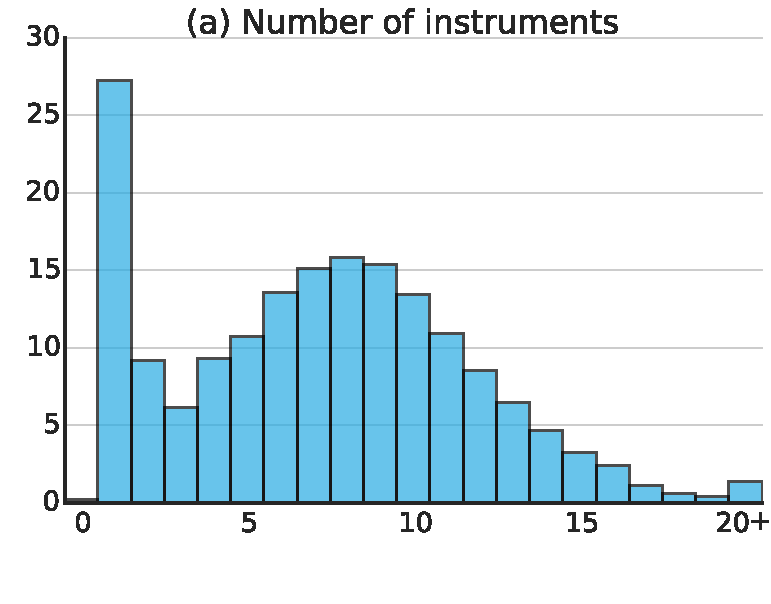
\includegraphics[width=\textwidth]{n_instruments.pdf}
    \end{subfigure}
    \begin{subfigure}{.23\textwidth}
        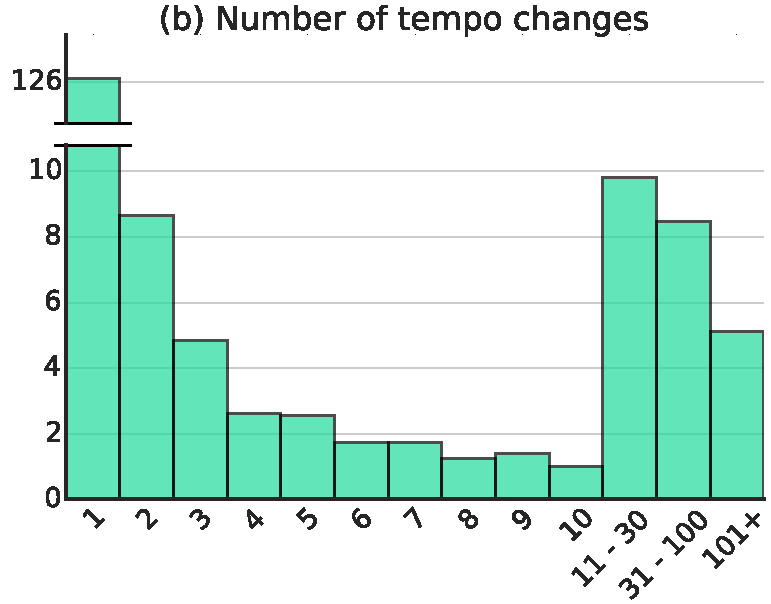
\includegraphics[width=\textwidth]{n_tempos.pdf}
    \end{subfigure}
    \begin{subfigure}{.23\textwidth}
        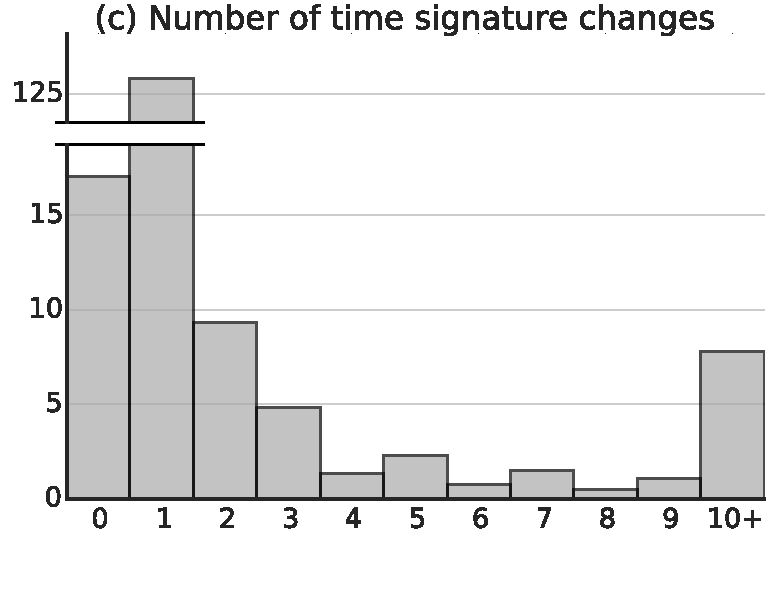
\includegraphics[width=\textwidth]{n_signatures.pdf}
    \end{subfigure}
    \begin{subfigure}{.23\textwidth}
        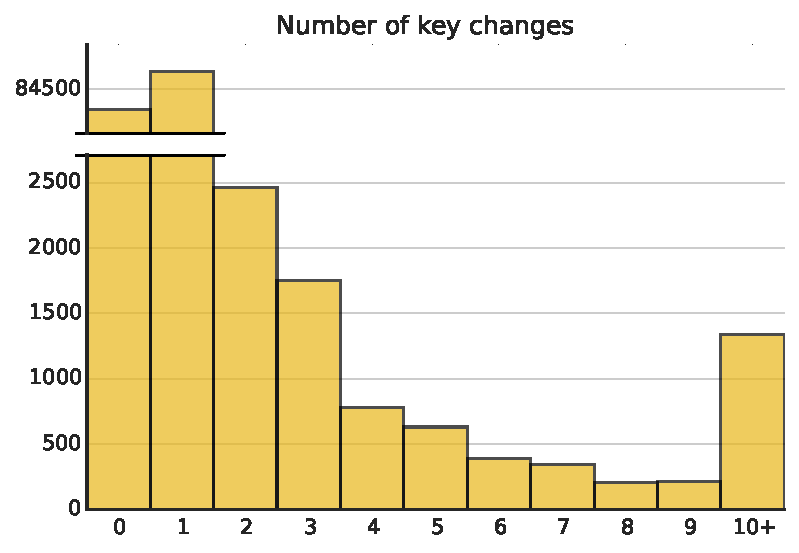
\includegraphics[width=\textwidth]{n_keys.pdf}
    \end{subfigure}

    \begin{subfigure}{.23\textwidth}
        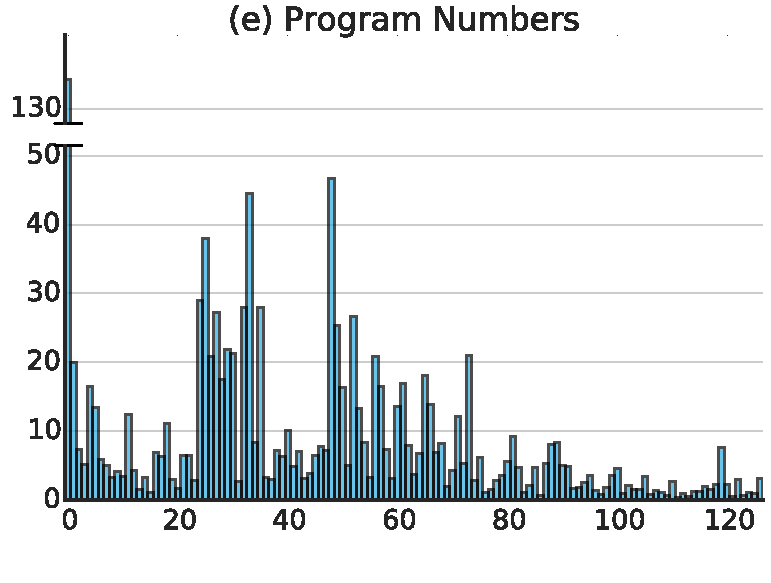
\includegraphics[width=\textwidth]{program_numbers.pdf}
    \end{subfigure}
    \begin{subfigure}{.23\textwidth}
        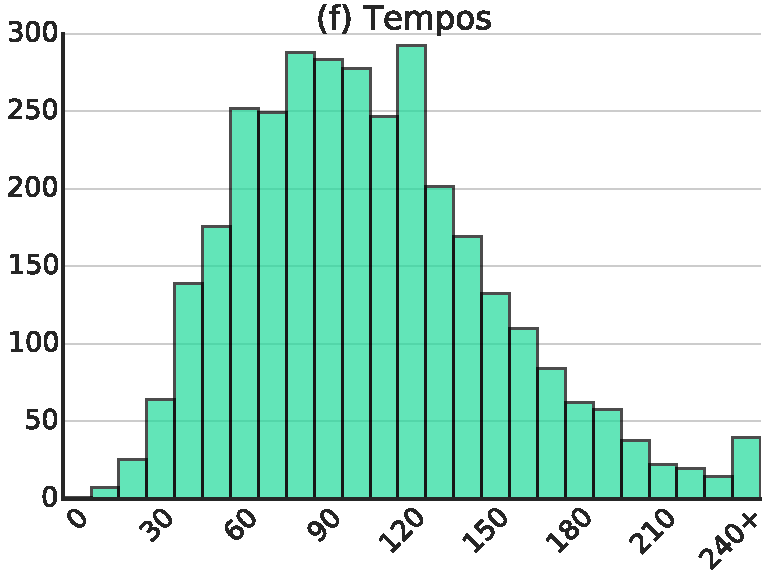
\includegraphics[width=\textwidth]{tempos.pdf}
    \end{subfigure}
    \begin{subfigure}{.23\textwidth}
        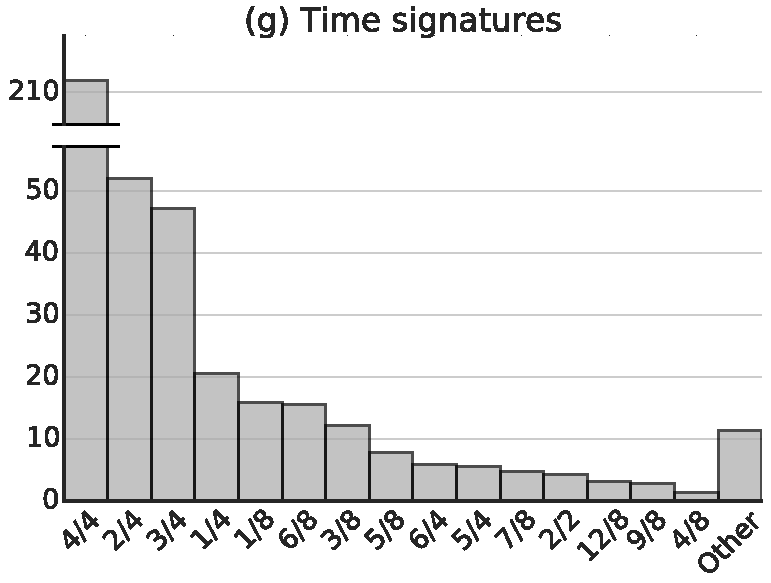
\includegraphics[width=\textwidth]{time_signatures.pdf}
    \end{subfigure}
    \begin{subfigure}{.23\textwidth}
        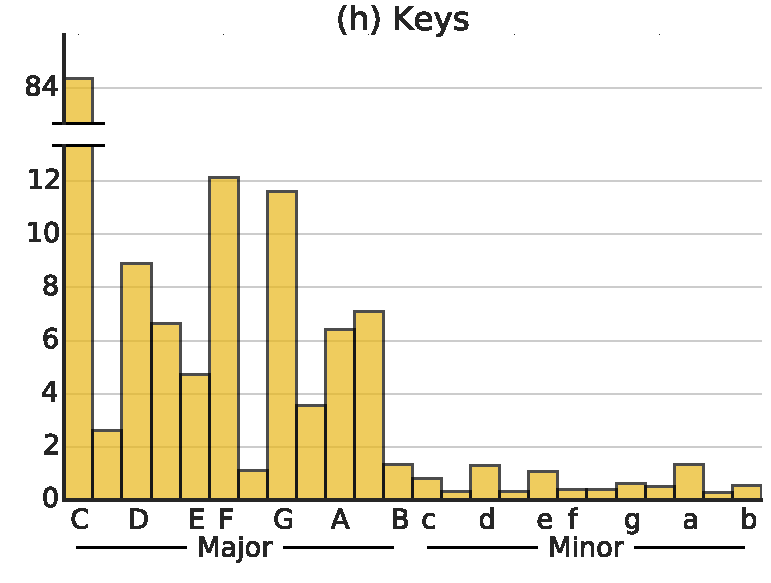
\includegraphics[width=\textwidth]{keys.pdf}
    \end{subfigure}
    \caption{Statistics about sources of information in 176,141 unique MIDI files scraped from the internet.
    Histograms in the top row show the number of MIDI files which had a given number of events for different event types; in the bottom row, we show distributions of the different values set by these events across all MIDI files.
    For example, about 125,000 MIDI files had a single time signature change event, and about 210,000 of the time signatures found in all of our MIDI files were 4/4.}
    \label{fig:statistics}
\end{figure*}

\subsection{Transcription}

MIDI files are specified as a collection of ``tracks'', where each track consists of a sequence of MIDI events on one of 16 channels.
Commonly used MIDI events are note on and note off messages, which together specify the start and end time of notes played at a given pitch on a given channel.
Various control events also exist, such as pitch bends, which allow for finer control of the playback of the MIDI file.
Program change events determine which instrument these events are sent to.
The General MIDI standard defines a correspondence between program numbers and a pre-defined list of 128 instruments.
The distribution of the total number of program change events (corresponding to the number of instruments) across the MIDI files in our collection and the distribution of these program numbers are shown in Figures \ref{fig:statistics}(a) and \ref{fig:statistics}(e) respectively.

This specification makes MIDI files naturally suited to be used as transcriptions of pieces of music, due to the fact that they can be considered a sequence of notes played on a collection of instruments.
As a result, many MIDI files are transcriptions and are thus commonly used as training data for automatic transcription systems (see \cite{turetsky2003ground} for an early example).
This type of data also benefits score-informed source separation methods, which utilize the score as a prior to improve source separation quality \cite{ewert2014score}.
An additional natural use of this information is for ``instrument activity detection'', i.e. determining when certain instruments are being played over the course of a piece of music.
Finally, the enumeration of note start times lends itself naturally to onset detection, and MIDI data has therefore been used for this task \cite{bello2005tutorial}.

\subsection{Musicological Features}

Because many MIDI files are transcriptions of music, they can also be used to compute high-level musicological characteristics of a given piece.
Towards this end, the software library jSymbolic \cite{mckay2006jsymbolic} includes functionality to extract a wide variety of features, including instrumentation, rhythm, and pitch statistics.
Similarly, music21 \cite{cuthbert2010music21} provides a general-purpose framework for analyzing collections of digital scores (including MIDI files).
Computing these features on a collection of MIDI transcriptions is valuable for omputational musicology and can enable data-driven corpus studies.
For example, \cite{cuthbert2011feature} discusses the use of music21 and jSymbolic to extract features from scores and use them to distinguish music from different composers and musical traditions.

\subsection{Meter}

Timing in MIDI files is determined by two factors: The MIDI file's specified ``resolution'' and tempo change events.
Each event within the MIDI file specifies the number of ``ticks'' between it and the preceding event.
The resolution, which is stored in the MIDI file's header, sets the number of ticks which correspond to a single beat.
The amount of time spanned by each tick is then determined according to the current tempo, as set by tempo change events.
For example, if a MIDI file has a resolution of 220 ticks per quarter note and the current tempo is 120 beats per minute,\footnote{Actually, tempo change events specify the number of microseconds per quarter beat, but this can be readily converted to beats per minute.} each tick would correspond to $60/(120*220) = 0.002\overline{27}$ seconds.
If a MIDI note-on event in this file is specified to occur 330 ticks after the previous event, then it would occur $330*0.002\overline{27} = .75$ seconds later.

The timing in a MIDI file can vary over time by including many tempo change events.
In practice, as shown in Figure \ref{fig:statistics}(b), most MIDI files only contain a single tempo change and are therefore transcribed at a fixed tempo.
However, there are many MIDI files in our collection which have a large number of tempo change events (as indicated by the rightmost bars in Figure \ref{fig:statistics}(b)).
We have found that this is a common practice for making the timing of a MIDI transcription closely match that of an audio recording of the same song.
Despite the fact that the default tempo for a MIDI file is 120 beats per minute, Figure \ref{fig:statistics}(c) demonstrates that a wide range of tempos are used.
In practice, we find that this is due to the fact that even when a single tempo event is used, it is often set so that the MIDI transcription's approximates that of an audio recording of the same song.

Time signature change events further augment MIDI files with the ability to specify time signatures, and are also used to indicate the start of a measure.
By convention, MIDI files have a time signature change at the first tick, although this is not a requirement.
Because time signature changes are relatively rare in western popular music, the vast majority of the MIDI files in our collection contain a single time signature change, as seen in Figure \ref{fig:statistics}(c).
Despite the fact that 4/4 is the default time signature for MIDI files and is pervasive in western popular music, a substantial portion (about half) included a non-4/4 time signature, as shown in Figure \ref{fig:statistics}(g).

Because MIDI files are required to include tempo information in order to specify their timing, it is trivial to extract beat locations from a MIDI file.
By convention, the first (down)beat in a MIDI transcription occurs at the first tick.
Determining the beat locations in a MIDI file is therefore a simple matter of computing beat locations starting from the first tick and adjusting the tempo and time signature according to any tempo change or time signature change events found.
Despite this capability, to our knowledge MIDI files have not been used as ground-truth for beat tracking algorithms.

\subsection{Key}

An additional useful event in MIDI files is the key change event.
Any of the 24 major or minor keys may be specified.
Key changes simply give a suggestion as to the tonal content and do not effect playback, and so are a completely optional metadata event.
As seen in Figure \ref{fig:statistics}(d), this results in many MIDI files omitting key change events altogether.
A further complication is that a disproportionate number (about half) of the MIDI files in our collection had key changes to the key of C major.
This disagrees with corpus studies of popular music, e.g. \cite{carlton2012analyzed} which found that only about 26\% of songs from the Billboard 100 were in C major.
We believe this is because many MIDI transcription software packaged automatically insert a C major key change at the beginning of the file.

\subsection{Lyrics}

Lyric meta events, .kar files

\subsection{What's Missing}

Explicit labeling of melody or voice instrument

Chords, segmentation

Metadata

\section{Utilizing MIDI Files as Ground Truth}
\label{sec:utilizing}

\subsection{Matching}

Required for nearly everything.

For small collections, you might not have to do anything.

For large collections, you need sophisticated methods because of lack of metadata.

Beneficial for MIDI analysis too, thanks to matching it with audio metadata collections.

\subsection{Aligning}

Required for all time-sensitive information.

\subsection{Evaluating Quality}

In some cases, the transcription may be bad.

\subsection{Extracting Information}

Short description of \texttt{pretty\_midi}.

\section{Measuring a Baseline of Reliability for MIDI-Derived Ground Truth}
\label{sec:measuring}

Match and align to Isophonics Beatles collection

\subsection{Beat Experiment}

\subsection{Key Experiment}

\section{Discussion}
\label{sec:discussion}

As-is, a lot of the information is usable.

Improving audio-to-MIDI alignment as a proxy for getting additional metadata.

Many additional avenues for improvement of measuring quality.

More information sources: Guitar Pro, MusicXML

\bibliography{refs}

\end{document}
